\appendix
\appendixpage
\addappheadtotoc

\section{Recovery Figures}

To visually demonstrate some limitations of this error correction scheme, the following figures show the use of Reed-Solomon codes to repair bitmap images.

Figure A has 12966 errors and can be repaired, yet figure B has only 3288 errors and cannot be repaired.
This is because the errors in figure A are one contiguous burst, whereas the errors in figure B are many small bursts spread across the image, damaging more blocks than in figure A.

Figure C is the recovered image from figure A.

See the script \texttt{generate\_figures.py} for how these images were generated.

\begin{figure}[H]
    \centering
    \begin{subcaptionbox}{A recoverable bitmap image with one corrupt area.}
        {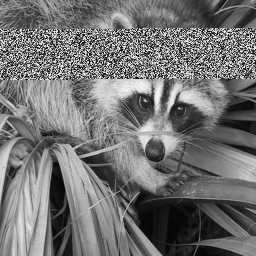
\includegraphics[width=0.3\textwidth]{face_2.png}}
    \end{subcaptionbox}
    \hfill
    \begin{subcaptionbox}{An unrecoverable bitmap image with many small corrupt areas.}
        {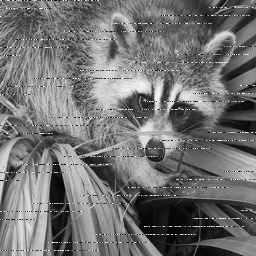
\includegraphics[width=0.3\textwidth]{face_3.png}}
    \end{subcaptionbox}
    \hfill
    \begin{subcaptionbox}{Figure A, repaired.}
        {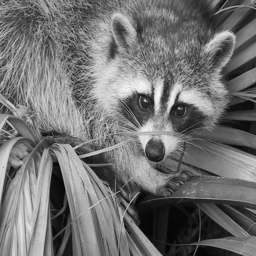
\includegraphics[width=0.3\textwidth]{face_2_repaired.png}}
    \end{subcaptionbox}
    
    \caption{Image source: \texttt{scipy.datasets.face} (derived from \url{https://pixnio.com/fauna-animals/raccoons/raccoon-procyon-lotor})}
\end{figure}
